\section{MMO}\label{sec:mmo}

In this section, we introduce the MMO (\motivation, \means, \oportunity) schema. We contend that a malicious device, just like a human criminal, needs Motive, Means, and Opportunity to perpetuate its attack. Using this schema, we can better understand the DMA vulnerabilities of an OS, the viability of possible DMA attacks, and their prevention. 

For example, using MMO schema, we are able to lay out the necessary conditions for a successful privilege escalation attack (i.e., code injection). Specifically, a malicious device needs all three prerequisites:
\begin{enumerate}
    \item \motivation: A kernel buffer filled with malicious code (e.g., a valid ROP attack) -- a \mabaf.
    \item \means: The kernel virtual address (\kva) of a \mabaf. Given the device is using \iova, the attacker needs to obtain the \kva{}, for example, by observing leaked pointers. 
    \item \oportunity: Write access to a known pointer, which can alter the CPU control flow. For example, write access to a data structure that holds a function callback pointer, at a known offset\footnote{The Linux kernel randomizes the layout of some data structures with \_\_randomize\_layout annotation \cite{rand_layout}.}.
\end{enumerate}

Another example is a full memory dump attack, which can be executed by merely having \oportunity. In this case, we are able to modify the kernel control flow in such a way as to cause it to dma\_map arbitrary kernel addresses at will. In order to achieve this, an attacker will need to modify a kernel pointer once before it is mapped and for a second time before send (i.e., TX) completion in order to avoid memory corruption (Section \ref{sec:linux_net}). 

To further emphasize the significance of the MMO attributes, we present a hypothetical scenario. Assume a NIC has write access to a page containing an RX packet (i.e., a received packet). Due to sub-page vulnerability and a random allocation coincidence, a structure with a callback pointer is inadvertently accessible with write permission. Also, the malicious device is able to create a valid \mabaf{} in the aforementioned page. It may seem that the device has a valid attack, whereas it actually lacks two essential prerequisites.

\begin{itemize}
    \item Missing \means: Without a valid \kva{} of the writable page, the device can not modify the callback function pointer to indicate the \mabaf.
    \item Missing \oportunity: Although a callback function pointer is available for modifications, the device has no way of knowing: 
    \begin{enumerate}
        \item[(a)] That a callback function pointer is available for sabotage.
        \item[(b)] The correct offset of the callback function pointer.
    \end{enumerate}
\end{itemize}

Under the hypothesized circumstance, and without additional information, a malicious device has practically no valid attack options. 
And while corrupting random kernel memory is still a possibility and may even cause a kernel panic \cite{MMT16}, it does not achieve the goal of privilege escalation.

\begin{figure}[t]
    \centering
    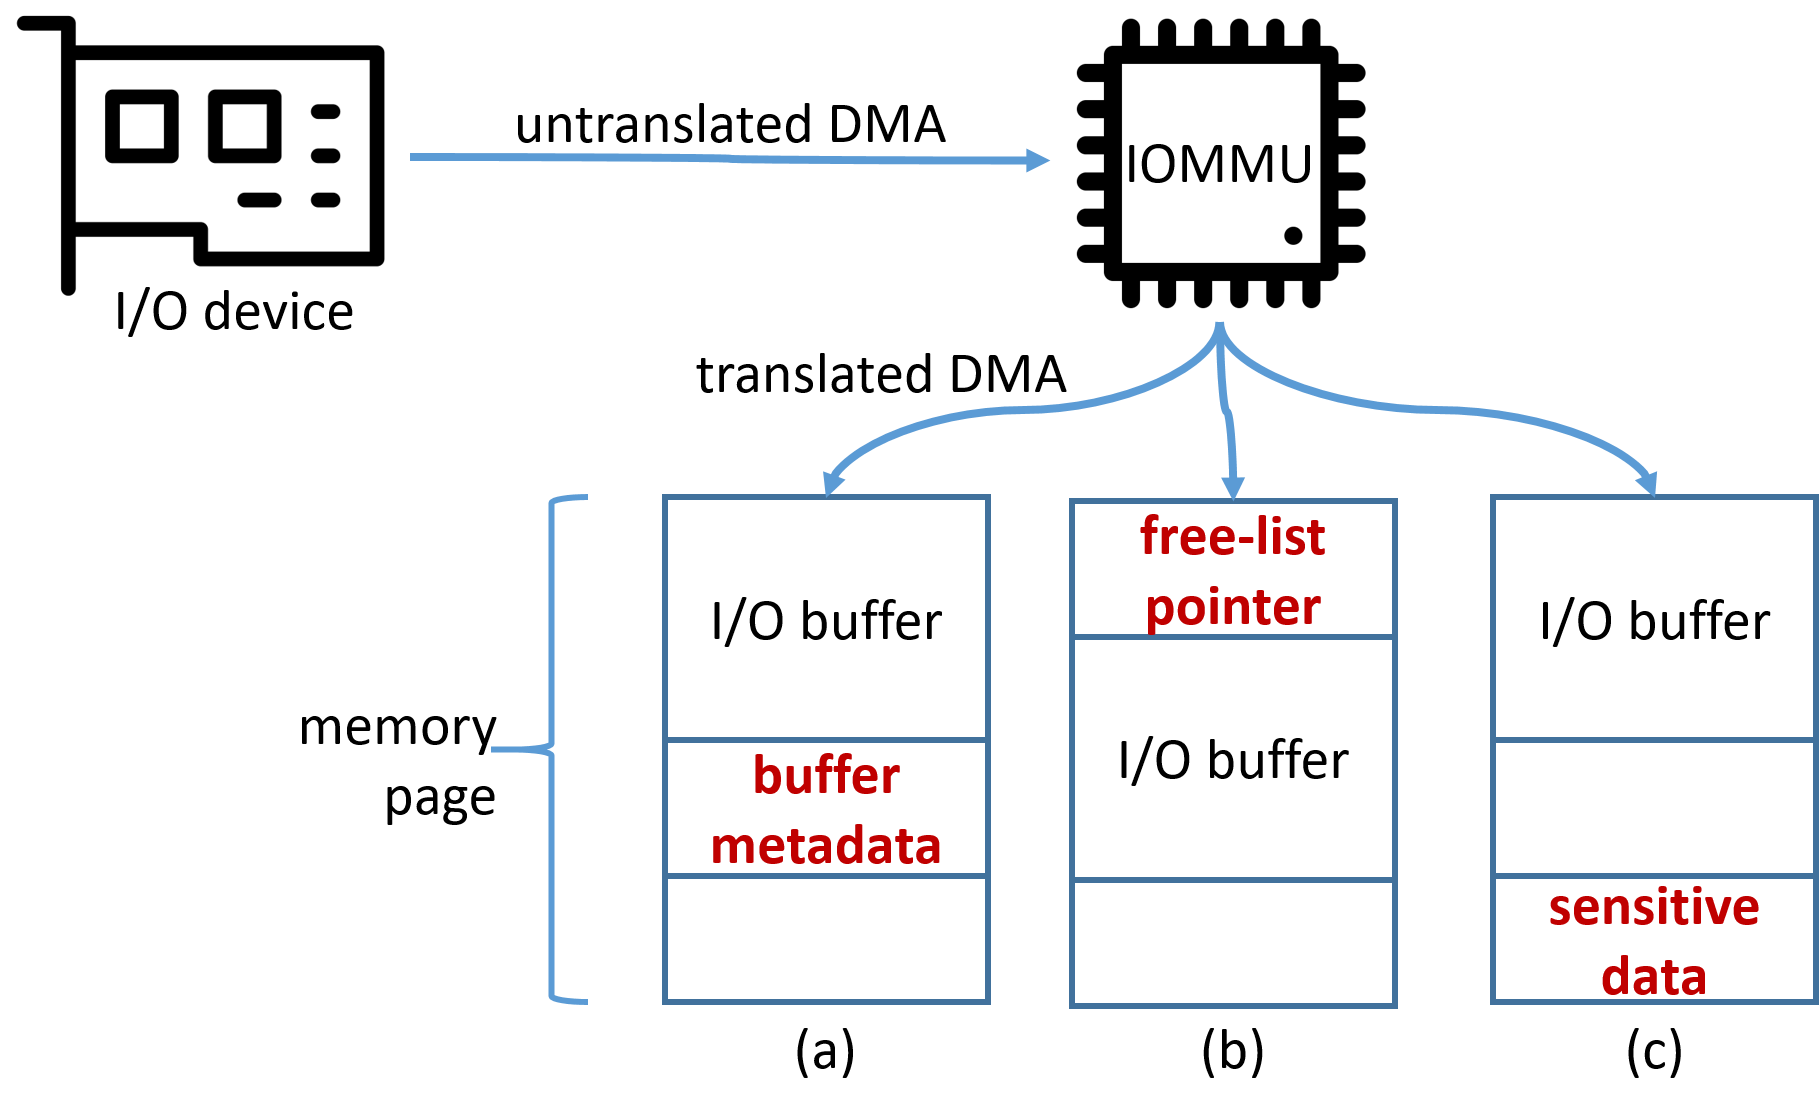
\includegraphics[width=1\columnwidth]{figs/colocation.png}
    \caption{\SV{TODO: update figure according to text and then update the caption accordingly.}Sub-page granularity DMA vulnerabilities when the I/O buffer resides in
a page that also holds other data: (a) I/O buffer metadata, (b) memory allocator’s
metadata such as free-list pointers and (c) randomly co-located sensitive buffers.}
    \label{fig:colocation}
\end{figure}

\begin{comment}
\subsection{Attack Mechanics}
Given that:
\begin{enumerate}
    \item IOMMU hardware is correctly implemented 
    \item IOMMU is correctly initialized and on time
\end{enumerate}
%One might assume that the systems are safe from DMA attacks. We contend that this is not the case. The \textit{least-privilege principle} requires that an entity such as a software module or a physical device must always have only the minimum necessary access to operate normally. In this chapter, we describe the risks caused by software when this principle is violated.
\end{comment}

\subsection{Static Analysis Tool}

Inspired by the MMO schema, we devise a static code analysis tool to classify device drivers by levels of risk. With well over a 1000 \texttt{dma\_map*} function calls, in the Linux Kernel alone, a manual process would be arduous.
Our static analysis tool flags drivers where \means{} or \oportunity{} are present. In the case of I/O devices \motivation{} is usually trivial as the device usually has a legitimate write access. The tool looks for \texttt{dma\_map*} functions and traces back the call stack to identify if the mapped buffer is embedded inside a data structure; additionally we look for functions (e.g \texttt{build\_skb}), that create a data structure inside a mapped buffer. The risk is classified according to the access permission, \motivation (indicated by READ) or \oportunity (indicated by WRITE/BIDIRECTIONAL). 
Finally, the output of the tool presents structured and filtered findings suitable for deeper human expert analysis to determine if a viable attack is feasible.

\subsection{Sub-Page Vulnerability}\label{sec:subpage}

Currently, the Linux kernel uses the same memory allocation mechanism (e.g., kmalloc) for both I/O buffers and regular kernel memory use. Consequently, I/O buffers often share pages with other, potentially sensitive, kernel buffers. Since IOMMU works in page granularity, the respective I/O devices gain access to these kernel buffers as well. 

We classify the different types of potentially co-located data, into three categories, as illustrated in Figure~\ref{fig:colocation}:

\begin{enumerate}
    \item[(a)] The I/O buffer is part of a bigger data structure. In some cases, this data structure may include function pointers.
    \item[(b)] The OS (e.g., memory allocator) rather than the driver saves metadata, such as free-lists, on the same page as the I/O buffer \cite{Cor07}. Manipulating these data structures may also compromise the system  \cite{ak09}.
    \item[(c)] The I/O buffer and another dynamically allocated memory may coincidentally reside in the same page. This common situation causes data leakage (e.g., kernel pointers).
     \item[(d)] The same page is mapped multiple times due to co-located device driver buffers. Resulting in multiple \iova{} for the same page.
\end{enumerate}

%In case (a),  
%Other fields in such data structures might be dangerous as well.
%We used randomly colocated pointers to break kASLR, as we discuss in Chapter 5. Why do OSs ignore the disparity between I/O buffer allocation alignment and protection granularity? One possible explanation is the benefits of dense memory allocations: lower internal memory fragmentation, which results in higher memory utilization, and lower translation lookaside buffer (TLB) pressure, which reduces the number of TLB misses. We suspect, however, that the main reason for the disparity is actually more prosaic. As IOMMUs were introduced to commodity servers relatively recently, OS developers have been reluctant to overhaul existing device drivers and change the way they allocate and manage their memory. Instead, IOMMU mapping operations were abstracted from device drivers, and implemented on top of existing DMA APIs [MHJ, The]. As a result, the memory allocation of I/O buffers has not been modified and adapted to take into consideration the IOMMU protection granularity.

\subsection{Deferred Invalidation vulnerability} 
\begin{figure*}[t]
    \centering
    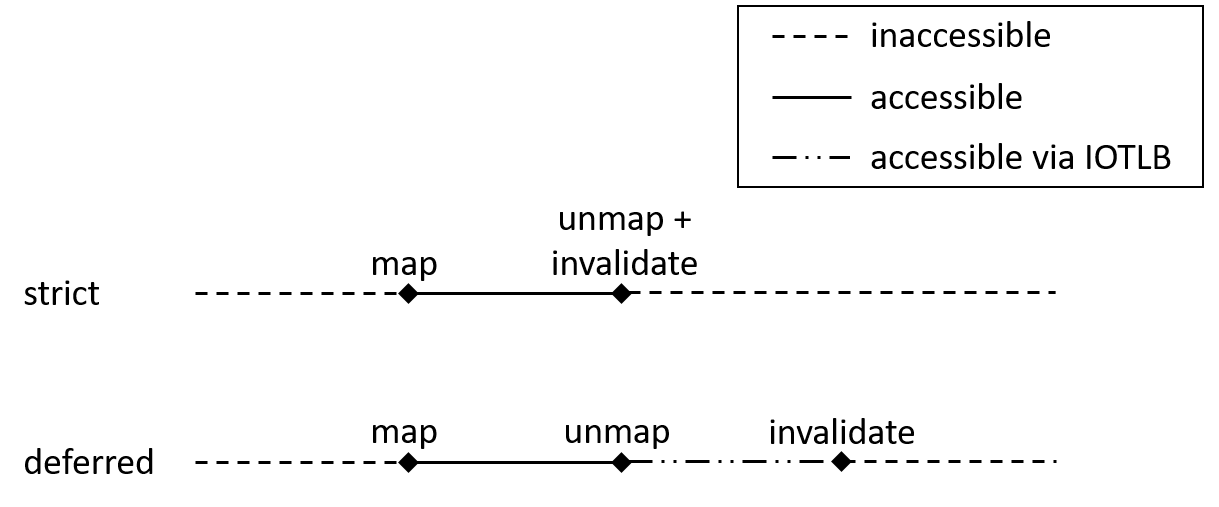
\includegraphics[width=1.3\columnwidth]{figs/deferred.png}
    \caption{Strict vs. deferred IOTLB invalidations. In deferred mode, there is a period
where the data is accessible but the mapping no longer exists.}
    \label{fig:deferred}
\end{figure*}
To translate addresses efficiently, the IOMMU caches translations in an input/output translation lookaside buffer (IOTLB). Like MMUs, IOMMUs do not maintain consistency between the IOTLB and the IOMMU page tables, which reside in memory; instead, the OS is required to restore consistency by explicitly invalidating the IOTLB. Therefore, to ensure that the IOTLB never holds stale entries, the OS must invalidate the IOTLB immediately after it removes memory mappings. Yet this scheme, called the “strict” mode in Linux, can degrade performance, as IOTLB invalidations can induce very high overhead \cite{MMT16,MSMT18,Peleg15}. In I/O intensive workloads, the number of required IOTLB invalidations can be extremely high, as IOMMU entries are unmapped following each I/O operation. Moreover, the overhead of each IOTLB invalidation can be as high as 2000 cycles \cite{ABYTS11}, considerably more than TLB invalidation, which takes roughly 100 cycles \cite{Han14}. To reduce this overhead, Linux defers TLB invalidations by default, and instead performs periodic global TLB invalidations. This “deferred” mode induces smaller performance overheads relative to the alternative “strict” mode. Nevertheless, as depicted in Figure \ref{fig:deferred}, deferring IOTLB invalidations may not prevent I/O devices from accessing unmapped pages, as the IOMMU may perform translations using stale IOTLB entries until the actual invalidation. This behavior introduces a security hazard, as the OS can reuse pages for other purposes after they are unmapped, regardless of the actual time of IOTLB invalidation. In the time window between the unmap operation and the actual invalidation, the OS may place sensitive data in the unmapped page-frame which the device may then read or modify. This time frame may be as high as 10 milliseconds when I/O traffic is low \cite{MSMT18}. In fact, this is a common scenario, as OSs prefer to reuse “hot” page-frames, recently freed, as they are likely to be already cached in the CPU caches\cite{hotcold}
. Therefore, it is possible in certain cases to predict how unmapped memory would be reused and which data it would expose.  
%As we demonstrate in Section 4.3, this behavior enables us to build robust assaults powerful enough to gain full control over a victim system.
\subsection{Threat Model}
Our attacks are built on the following assumptions:
\begin{enumerate}
    \item The actual attack is performed by a DMA-capable malicious device.
    \item There is software that violates the least-privilege principle with respect to the I/O device. The inherent vulnerabilities in the common use of the IOMMU make this a realistic assumption (§\ref{sec:sbp2_attack}). 
 \end{enumerate}
 The attacks discussed in this work are not executed by modifying the victim’s OS or drivers. We also assume that any hardware aside from the specific malicious device is working as expected, especially the DMA controller and the IOMMU itself. We also do not consider ports intended for debugging (e.g., jtag).
\subsection{Consequences}
The greatest potential consequence of our attacks is privilege escalation, which allows attackers to execute arbitrary code with kernel privileges. In all our experiments, we successfully executed code in the context of the kernel. Another, potential consequence is full system memory; these are harder to thwart and even harder to detect.  
Lastly, a consequence of a simple attack is denial of service \cite{MMT16}; where we crush the OS. Ideally, malformed devices should not be able to crash the entire system. The IOMMU is expected to properly isolate the devices from the OS to ensure this does not happen. Bad isolation, such as colocation of different types of data in the same page, may lead to system instability. To reach the above results, the attacker must have write permissions to some memory region. When an attacker has only read permissions, the consequences may still be interesting as they may lead to data leakage\cite{thunder}. The kernel often keeps sensitive data such as encryption keys and passwords as plain-text in memory. Attackers may use incorrect read permissions to leak this sensitive information.